% show rdfs of the ab initio & classical runs for malonic

% talk about similarities and differences

% suggest the deficiency in the classical, and how a better model should be developed to capture that first peak on the alcohol.
\begin{figure}[h!]
	\begin{center}
		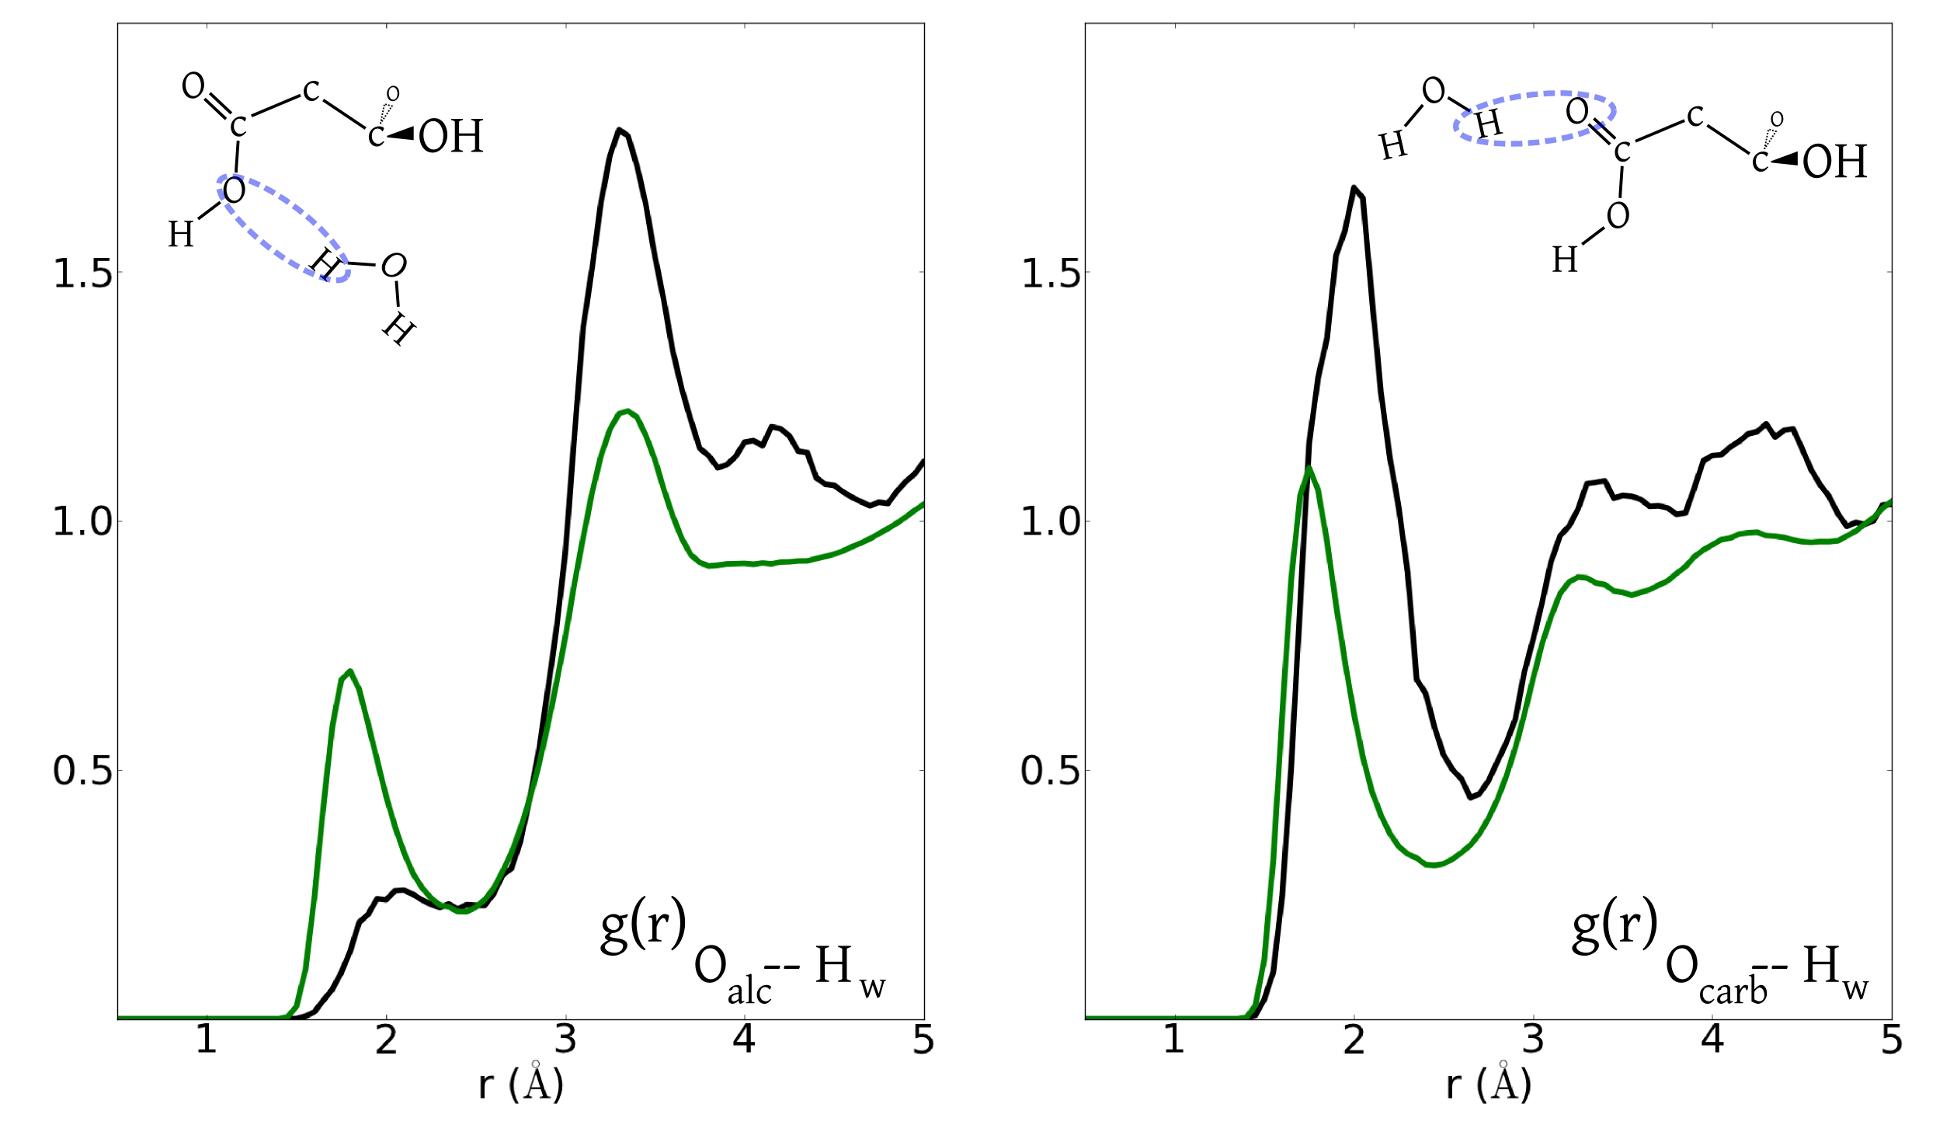
\includegraphics[scale=1.0]{images/rdf/MalonicRDF-small.png}
		\caption{Radial distribution functions, g(r), were calculated for the pair correlations between the acid oxygens and water hydrogen atoms. The acid alcohol moiety oxygen - water hydrogen RDF (left) and the carbonyl oxygen - water hydrogen RDF (right) are plotted. Each RDF is shown for both the ab initio simulations of the present study (black), and for classical MD simulations (green) taken from a data set used for a recently published study by our group.\cite{Blower2012}}
		\label{fig:rdf}
	\end{center}
\end{figure}
